\scanpage{11}
\mspage{1}

Hypercoverings.

Let $\mathcal X$ be a $\mathcal U$-topos category. We want to define \deleted{\unsure{a}} the notion of a \uline{hypercovering} of $\mathcal X$ (or again, of the topos defined by $\mathcal X$), indexed by a small category $A$. \deleted{Such a hypercovering} This will by definition be a functor
\diagram{\begin{tikzcd}[ampersand replacement=\&,row sep=small]
\varphi:\quad A\arrow[r]\&\mathcal X\\
\alpha\arrow[r,mapsto]\&U_\alpha\ (=\unsure{\varphi|\varphi_{\mathcal X}}(\alpha))
\end{tikzcd}}
, satisfying certain conditions, inspired by \unsure{the|the} 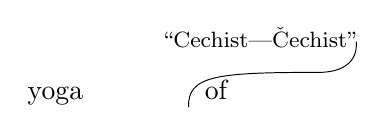
\begin{tikzpicture}[baseline=(yogab.base),x=1cm,y=1cm]
\node[anchor=base west,inner sep=0pt] (yogab) at (0,0) {yoga};
\node[anchor=base west,inner sep=0pt] at (2.25,0) {of};
\node[anchor=base west,inner sep=0pt,font=\footnotesize] at (1.70,.66) {\inserted{``\unsure{Cechist|\v{C}echist}''}};
\draw[line width=.35pt] (2.05,-.10) .. controls (2.04,.30) and (2.40,.34) .. (3.70,.34)
 .. controls (4.02,.34) and (4.20,.48) .. (4.18,.73);
\end{tikzpicture} coverings \unsure{and of} their nerves, and the refinement of this y.g. suggested by Cartier (for non-paracompact topological spaces). Here are the conditions that come to mind:

\uline{Hypothesis 1} The objects $U_\alpha$ ($\alpha\in\mathrm{Ob}\,A$) cover the terminal \unsure{object|object} $e_{\mathcal X}$ of $\mathcal X$.

\deleted{\uline{Hypothesis 1'} For every $\alpha_0\in\mathrm{Ob}\,A$, the induced functor $A/\alpha_0\longrightarrow\mathcal X/U_{\alpha_0}$ satisfies Hypothesis 1, i.e. the set of arrows $U_\alpha\longrightarrow U_{\alpha_0}$, associated with the arrows $\alpha\longrightarrow\alpha_0$ with target $\alpha_0$ in $A$,}
\margin{Is satisfied tautologically!}
\margin{10}
